\subsection{Убираем низкие частоты}

\def\num{15}
\def\a{3}
\def\from{-2}
\def\to{4}
\def\b{0.3}
\def\c{1}
\def\d{10}
\def\T{10}
\def\imageclip{8}


\subsubsection{Рассматриваемая функция}
Рассмотрим функцию $g(t)$ при параметрах $a=$~\a, $t1 =$~ \from, $t_2 =$~\to ~(см. рисунок~\ref{fig:wave_function_\num}) 
и ее \textit{зашумленную} версию $u(t)$ с параметрами $b =$~\b, $c =$~\c, $d =$~\d ~(см. рисунок~\ref{fig:noised_wave_function_\num}).
на промежутке $[-T/2,~T/2]$ с $T =$~\T.

\FloatBarrier
\subsubsection{Графики рассматриваемой и зашумленной функции}
\begin{figure}[ht!]
    \centering
    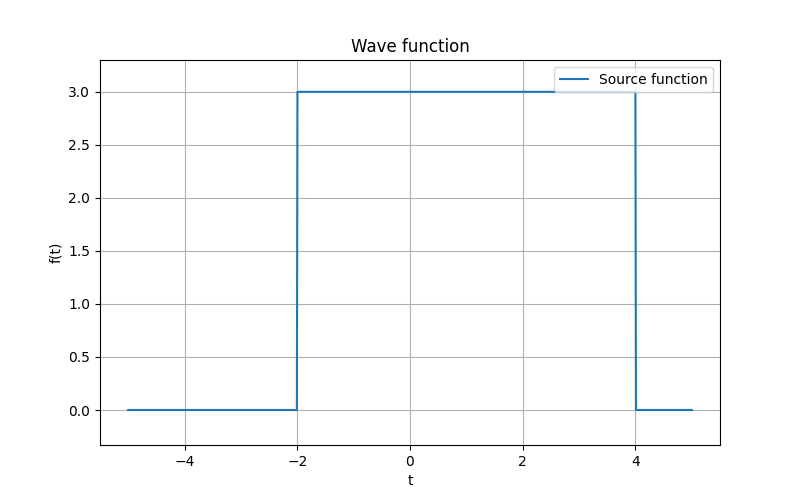
\includegraphics[width=\textwidth]{../results/\num/wave_function.png}
    \caption{Функция $g(t)$ с параметрами $a = \a$, $t_1 = \from$, $t_2 = \to$}
    \label{fig:wave_function_\num}
\end{figure}

\begin{figure}[ht!]
    \centering
    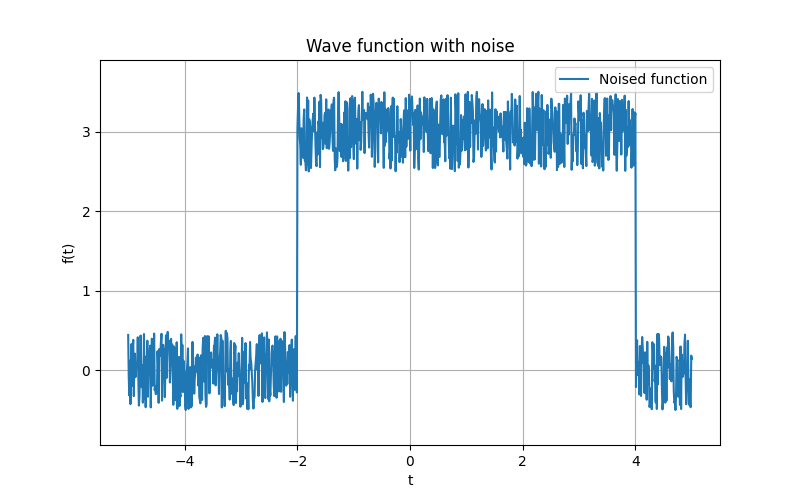
\includegraphics[width=\textwidth]{../results/\num/noised_wave_function.png}
    \caption{Функция $u(t)$ с параметрами $b = \b$, $c = \c$, $d = \d$}
    \label{fig:noised_wave_function_\num}
\end{figure}

\FloatBarrier
\subsubsection{Нахождение образов исходной и зашумленной функций}
Найдем образы исходной (см. рисунок~\ref{fig:wave_function_image_\num}) 
и зашумленной (см. рисуно~\ref{fig:noised_wave_function_image_\num}) функций с помощью преобразования Фурье. 

\begin{figure}[ht!]
    \centering
    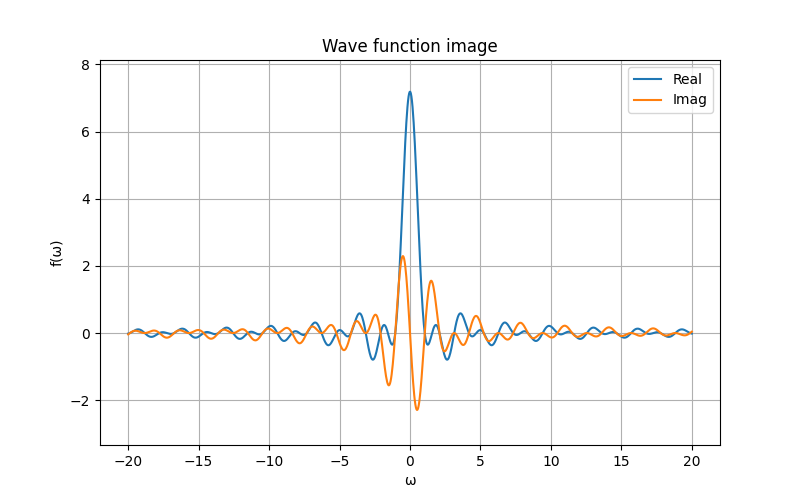
\includegraphics[width=\textwidth]{../results/\num/wave_function_image.png}
    \caption{Образ функция $g(t)$ с параметрами $a = \a$, $t_1 = \from$, $t_2 = \to$}
    \label{fig:wave_function_image_\num}
\end{figure}

\begin{figure}[ht!]
    \centering
    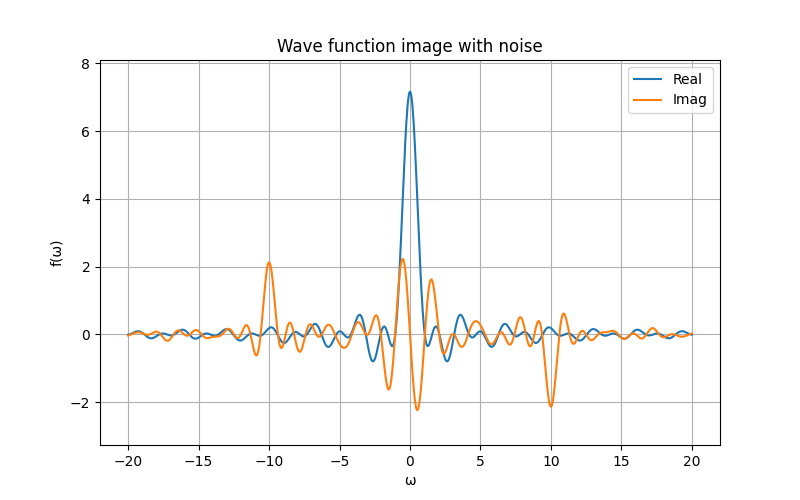
\includegraphics[width=\textwidth]{../results/\num/noised_wave_function_image.png}
    \caption{Образ функция $u(t)$ с параметрами $b = \b$, $c = \c$, $d = \d$}
    \label{fig:noised_wave_function_image_\num}
\end{figure}

Как и в прошлом случае, видим, что на графике образа зашумленной функции появились пики, которые отсутствуют на графике образа исходной функции.

\FloatBarrier
\subsubsection{Фильтрация низких частот}
\textit{Обрежем} образ функции $u(t)$, убрав компоненты, соответствущие низким частотам (см. рисунок~\ref{fig:noised_wave_function_image_clipped_\num}).

\begin{figure}[ht!]
    \centering
    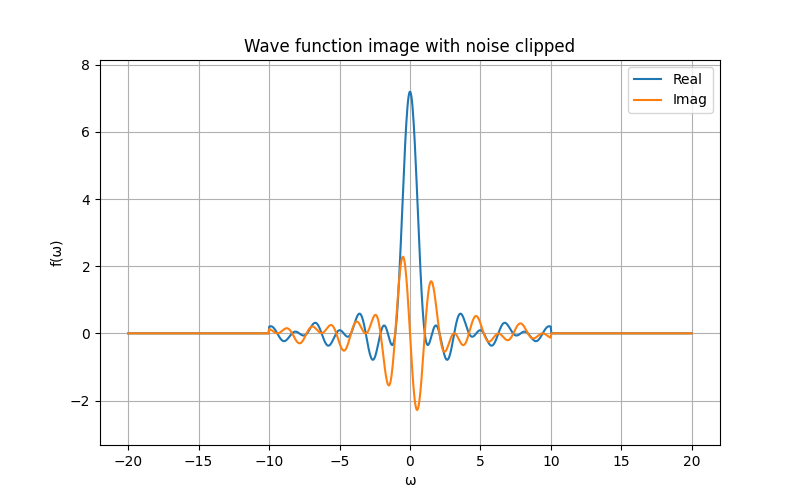
\includegraphics[width=\textwidth]{../results/\num/noised_wave_function_image_clipped.png}
    \caption{Обрезанный образ функция $u(t)$ при $\omega_0=$~\imageclip}
    \label{fig:noised_wave_function_image_clipped_\num}
\end{figure}

Как и ожидалось, низкочастотные компоненты ($|\omega| < \omega_0$) стали равны нулю. 

Теперь выполним обратное преобразование Фурье (использую обрезанный образ), получив при этом фильтрованную версию функции (см. рисунок~\ref{fig:wave_function_clipped_restored_\num}).

\begin{figure}[ht!]
    \centering
    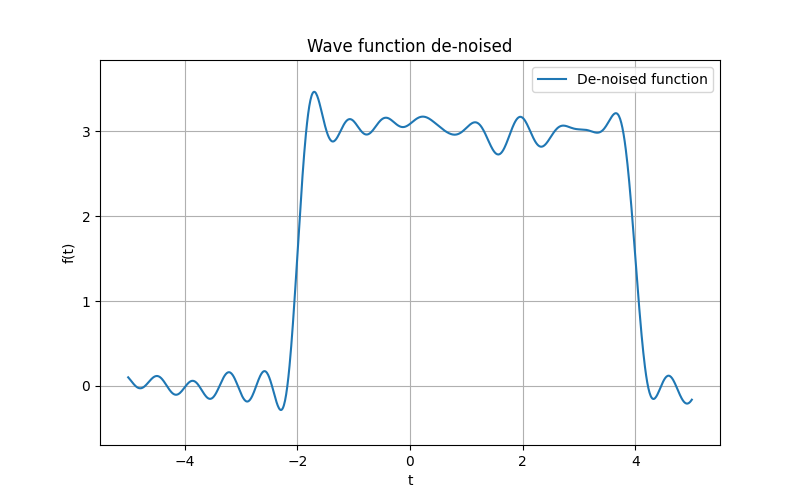
\includegraphics[width=\textwidth]{../results/\num/wave_function_clipped_restored.png}
    \caption{Фильтрованная функция $u(t)$ при $\omega_0=$~\imageclip}
    \label{fig:wave_function_clipped_restored_\num}
\end{figure}

Сравнительные графики исходной и фильтрованной функций представлены на рисунке~\ref{fig:wave_function_comparison_\num}. 
\begin{figure}[ht!]
    \centering
    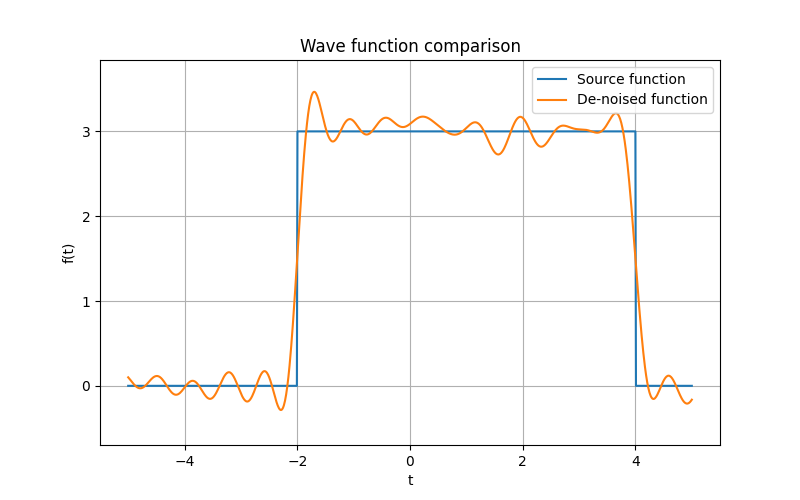
\includegraphics[width=\textwidth]{../results/\num/wave_function_comparison.png}
    \caption{Исходная и фильтрованная функция при $\omega_0=$~\imageclip}
    \label{fig:wave_function_comparison_\num}
\end{figure}

Видно, что от исходной функции остался только шум, что логично, ведь мы убрали низкие частоты, которые, в большинстве, и соответствовали самой функции.
Амплитуда шума осталась неизменной. 

